
Laskuvarjoon vaikuttaa useita erilaisia fysikaalisia voimia, jotka määräävät sen käyttäytymisen. Nämä voimat määräävät varjon lentosuunnan sekä etenemisnopeuden. Hyppääjä voi tietyssä määrin hetkellisesti vaikuttaa varjoon vaikuttaviin voimiin ja ennen kaikkea niiden suuntaan, mutta fysiikan peruslakeja ei hyppääjä (valitettavasti) voi kumota.  


\begin{Figure}\centering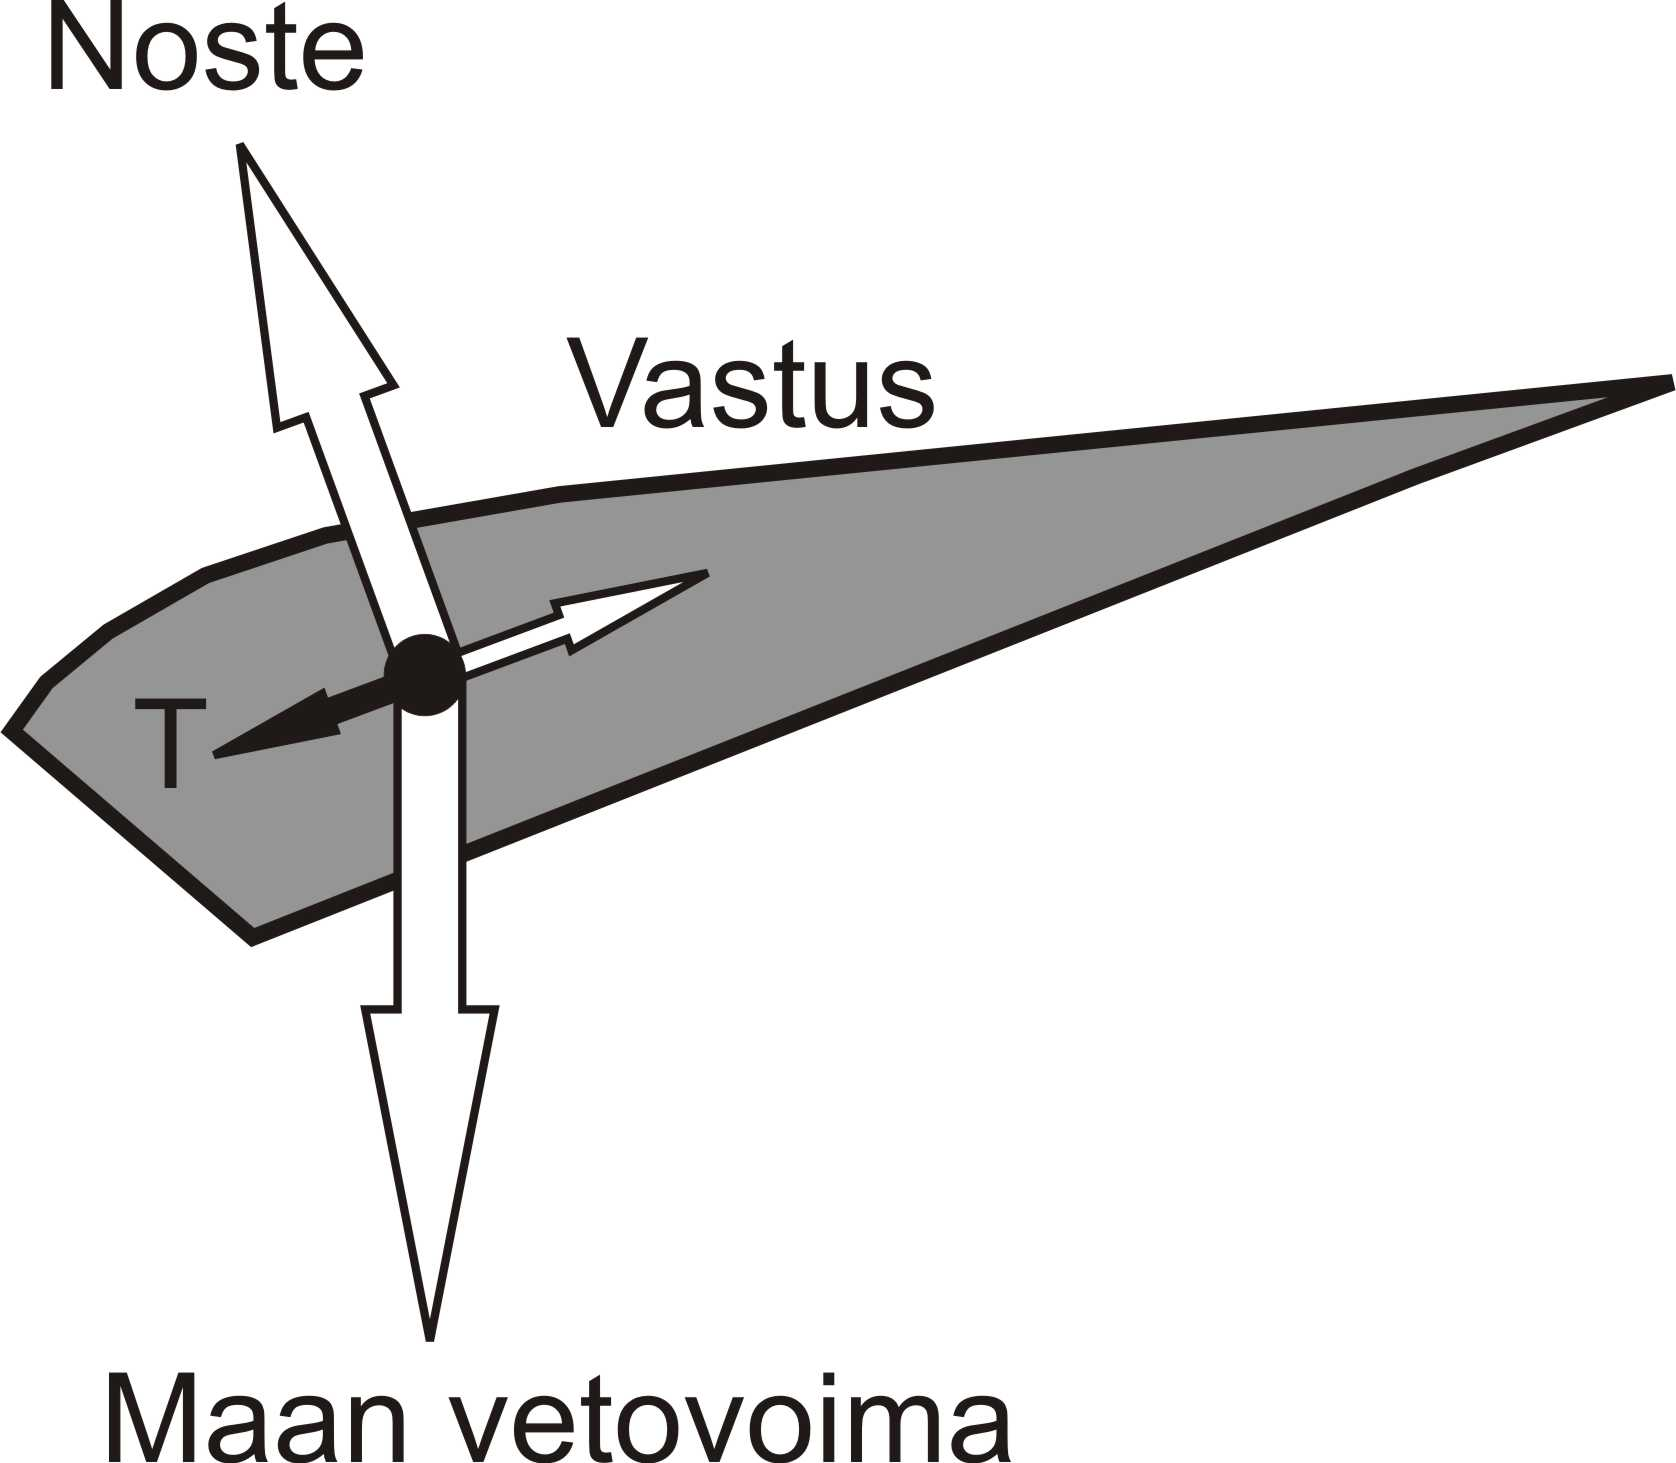
\includegraphics[width=0.7\textwidth]{Voimakuvio.jpeg}\captionof{figure}{Laskuvarjoon vaikuttavat voimat vakaassa lentotilassa.}\end{Figure} 


Kuten aikaisemmin on todettu, laskuvarjoa jarruttava voima on \textbf{vastus}. Laskuvarjon \textbf{kokonaisvastus} (drag) koostuu varjojärjestelmän ilmanvastuksesta, muotovastuksesta sekä indusoidusta vastuksesta. Vastusta voidaan vähentää huomattavasti erilaisilla teknisillä ratkaisuilla, mutta kokonaan vastusta ei järjestelmästä voida eliminoida. Lentolaitteissa eteenpäin vievää voimaa kutsutaan työntövoimaksi. Lentokoneessa työntövoima saadaan aikaan moottoreilla. Koska laskuvarjossa ei ole moottoreita, ilmanopeus ja \textbf{noste} (lift) muodostuvat laskuvarjon liitokulman (taittaa ilmaa) ja laskuvarjojärjestelmään (sekä sen alla roikkuvaan hyppääjään) vaikuttavan \textbf{maan vetovoiman} (gravity) avulla. Näin aikaansaadaan myös vastuksen kumoamiseen tarvittavaa \textbf{työntövoimaa} (thrust) nosteen eteenpäin suuntautuvan komponentin ja maan vetovoiman alaspäin suuntautuvan voiman resultanttina. Laskuvarjon ollessa stabiilissa lentotilassa (eli sillä ei ole kiihtyvyyttä mihinkään suuntaan) on näiden voimien summa nolla. Nosteen voidaan myös ajatella syntyvän aerodynaamisena nosteena Bernoullin lain mukaisesti siipiprofiilin aiheuttaessa paine-eron siiven ylä- ja alapuolille virtauksien nopeuserojen tuloksena (yläpinnalla alipaine). 


Mitä enemmän laskuvarjon alle laitetaan massaa (eli siis lisätään maan painovoimaa), sitä enemmän varjolle kehittyy myös ilmanopeutta. Mitä enemmän varjolla on ilmanopeutta, sitä enemmän se muodostaa nostetta. Painon määrää laskuvarjon alla kuvataan \textbf{siipikuormalla}. Ajateltaessa siipikuormaa kuvitellaan usein, että siipikuorma on vakio lentotilasta riippumatta. Näin ei kuitenkaan ole. Radikaali käännös lisää hetkellisesti siipikuormaa johtuen keskipakoisvoimasta. Ajatellaan vaikkapa narun päässä pyörivää painoa: mitä nopeammin paino pyörii, sitä suurempi jännitys narussa tarvitaan, jotta paino pysyy radallaan. Sama voima vaikuttaa myös hyppääjään voimakkaassa käännöksessä tai jarrutuksessa. Voimakkaan käännöksen aikana hyppääjä heilahtaa voimakkaasti kuvun sivulle ja aiheuttaa keskipakoisvoiman ansiosta hetkellistä siipikuorman kasvua varjossa. Tiettyyn rajaan asti voidaan ajatella, että suurempi paino laskuvarjon alla lisää varjon teoreettista suorituskykyä, koska varjon kehittämä fysikaalinen noste lisääntyy neliön suhteessa sen nopeuteen. Käytännössä siis 60 km/h kulkeva varjo kehittää neljä kertaa enemmän nostetta, sekä myös vastusta,kuin 30 km/h kulkeva varjo. Tästä syystä pienillä kuvuilla hypättäessä voidaan käyttää isompaa siipikuormaa. Kuitenkin kaikella tällä nopeuden lisäämisellä on haittapuolensa, joita käsitellään myöhemmin puhuttaessa varjon lentämisestä ja eri siipikuormista. 

\section{ Laskuvarjon liitokulma ja siihen vaikuttavat tekijät }
\label{laskuvarjoon-vaikuttavat-fysikaaliset-voimat-ja-nosteen-syntyminen-laskuvarjon-liitokulma-ja-siihen-vaikuttavat-tekijat}


Laskuvarjon punokset pitenevät punosryhmittäin (A\mbox{-,} B\mbox{-,} C- ja D-punokset) takahelmaa kohti. Tällä punostrimmillä (rigging angle) kupu saadaan lentämään tietyssä kulmassa. Tätä horisontin ja kuvun jänteen välistä kulmaa kutsutaan kuvun \textbf{asetuskulmaksi} (angle of incidence). Varjon asetuskulmaa voidaan lennettäessä muuttaa (jyrkentää tai loiventaa) vain kantohihnoista alas vetämällä. Etummaisista kantohihnoista vetämällä asetuskulma suurenee ja takimmaisista pienenee. Asetuskulma asettaa siipiprofiilin jänteen tiettyyn kulmaan ilmavirran (relative wind) kanssa, ja tätä kulmaa kutsutaan \textbf{kohtauskulmaksi} (angle of attack). 


\begin{Figure}\centering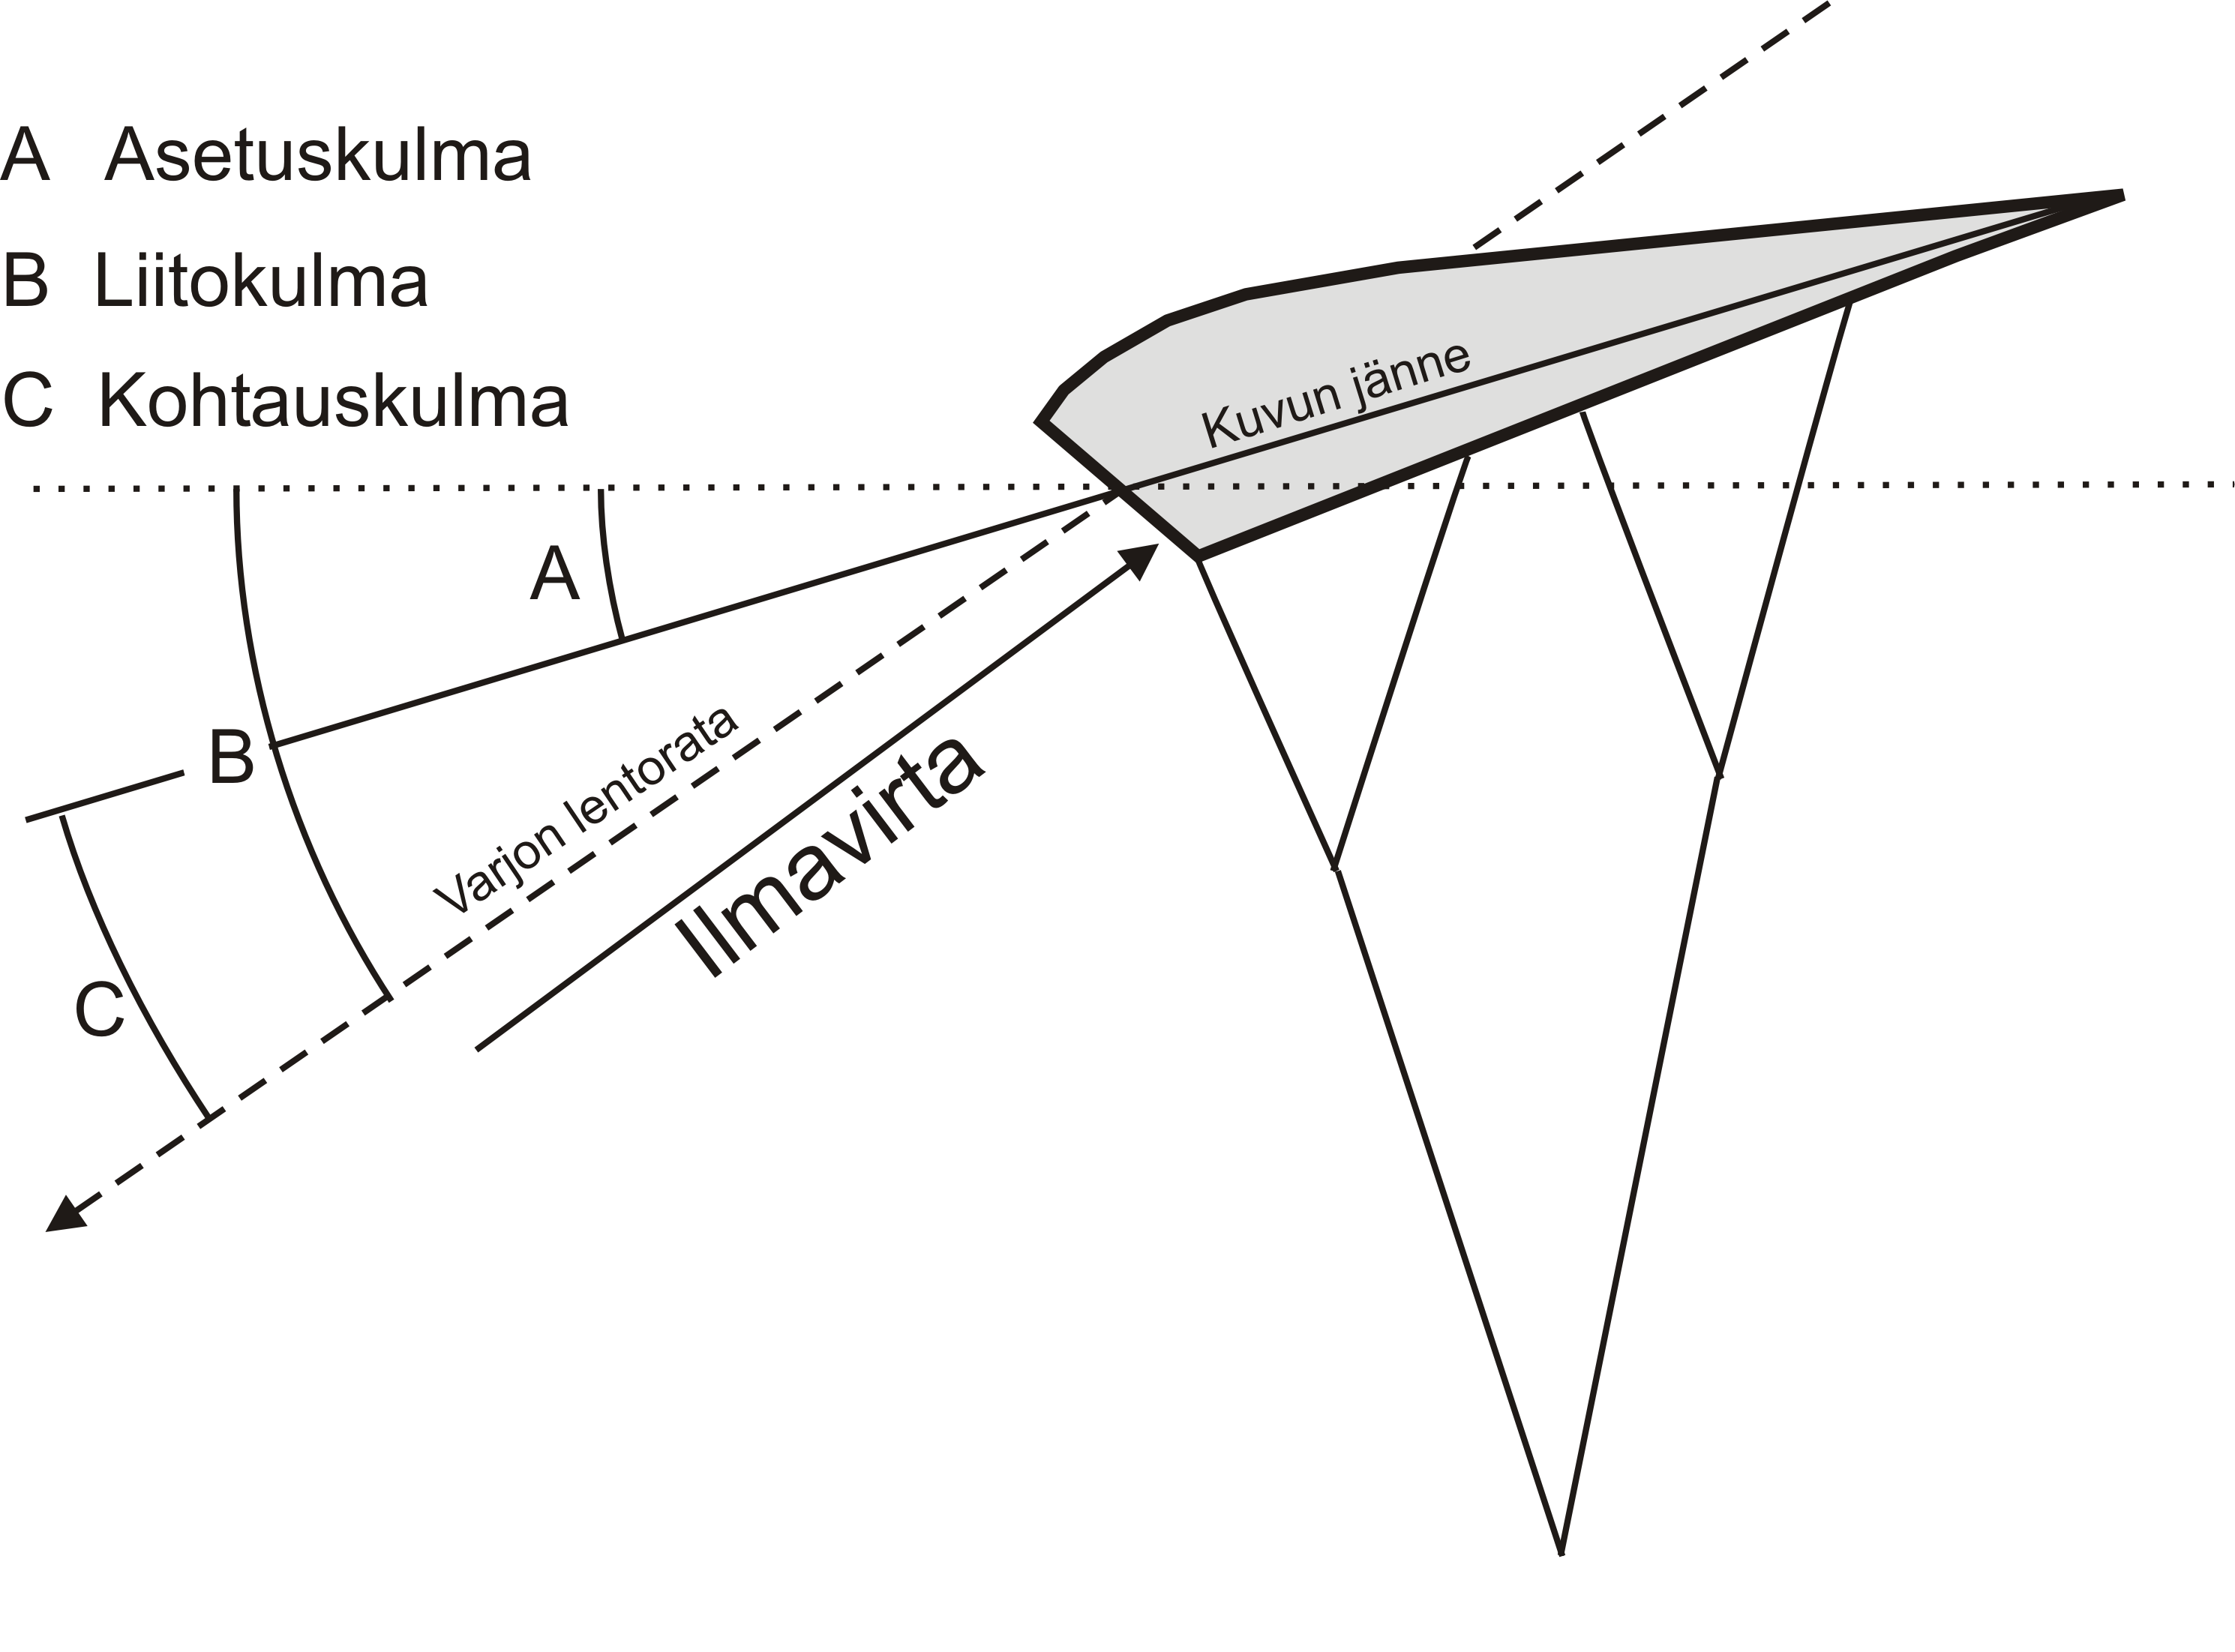
\includegraphics[width=0.99\textwidth]{Laskuvarjon_kulmat.png}\captionof{figure}{Laskuvarjon kulmat}\end{Figure} 


Kohtauskulma on kuvun jänteen ja siihen osuvan ilmavirran välinen kulma. Laskuvarjon kohtauskulmaa voidaan muuttaa joko jarruttamalla varjoa tai siirtämällä painopisteen sijaintia kuvun alapuolella.  


\begin{figure*}[]\centering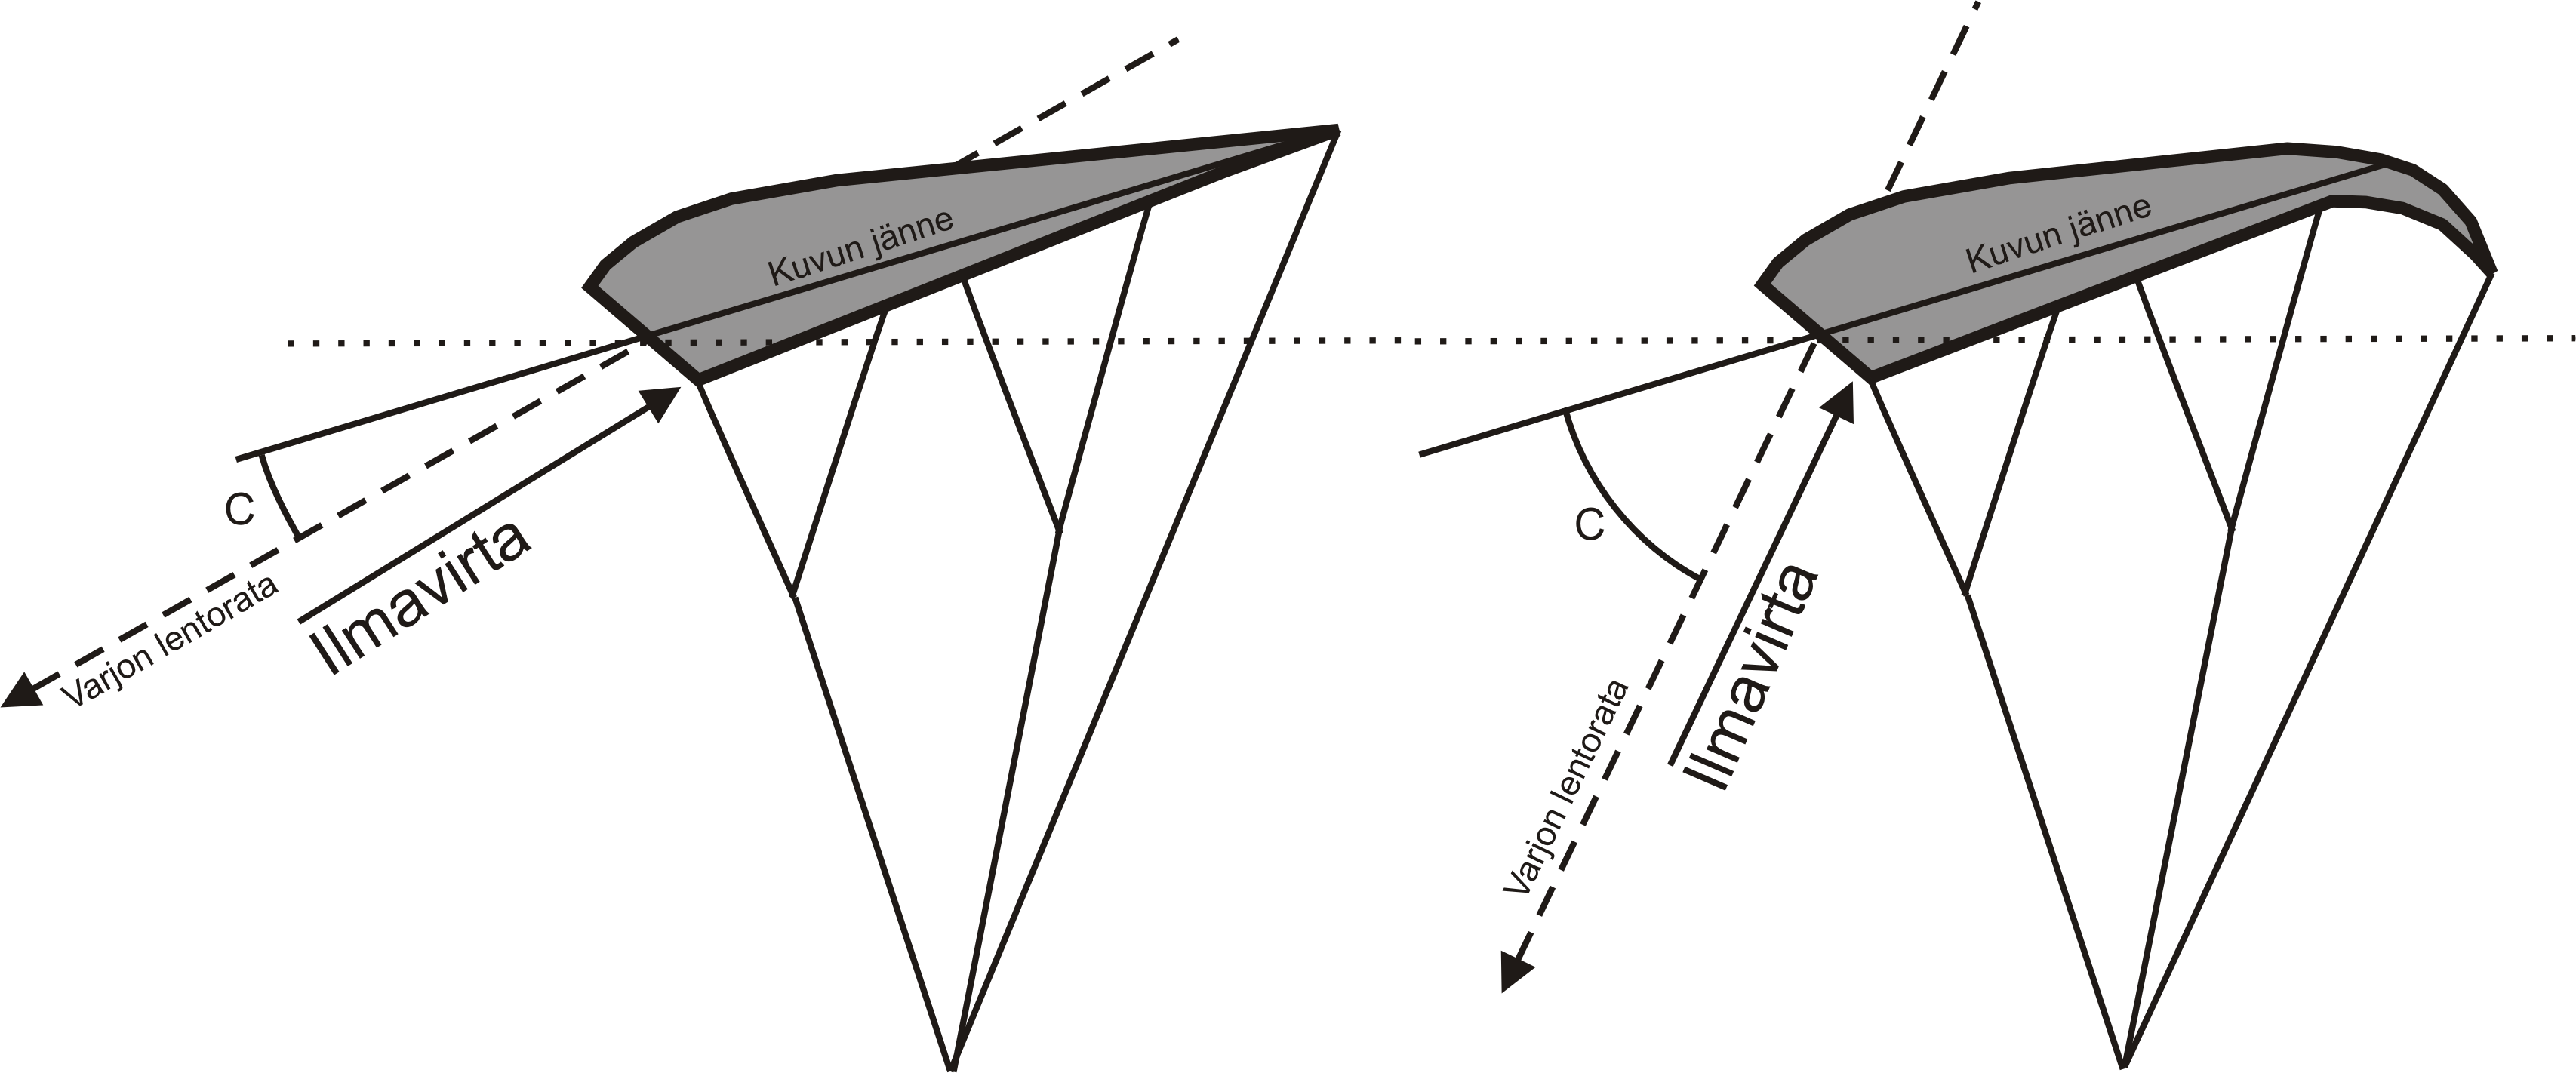
\includegraphics[width=0.9\textwidth]{Kohtauskulma.png}\caption{Kohtauskulma (C) ja sen muuttuminen lisättäessä jarruja}\end{figure*} 


Kohtauskulmaa voi muuttaa myös nopeilla ohjausliikkeillä, joko jarruja tai kantohihnoja käyttäen. Nopea ohjausliike aiheuttaa varjon liikesuunnan nopean muuttumisen. Punoksien päässä oleva hyppääjä ei kuitenkaan liikemomenttinsa vuoksi voi seurata muutosta välittömästi, vaan saa aikaan heiluriliikkeen. Kun painopiste siirtyy kuvun alla eteenpäin (nopea jarrutus tai veto takimmaisista kantohihnoista), kohtauskulma suurenee ja varjo fleeraa. Kun painopiste siirtyy taaksepäin (nopea jarrujen vapautus, nopea veto etummaisista kantohihnoista), varjo syöksähtää eteen- ja alaspäin. Vastaavat ilmiöt toteutuvat myös käyttämällä vain toisen puolen jarrua/kantohihnoja. Tällöin painopiste heilahtaa eteen/taakse suunnan lisäksi myös sivulle aiheuttaen kuvun kallistumisen ja kääntymisen.  


\textbf{Liitokulma} (glide angle, glide slope) on varjon lentoradan ja horisontin välinen kulma. Se määrittää varjon liitosuhteen, eli sen, kuinka paljon varjo lentää eteenpäin suhteessa menetettyyn korkeuteen. Eri lentotiloissa varjojen liitosuhteet vaihtelevat noin 2:1 ja 3:1 välillä. Tarkkoja liitokulmia ei ole valmistajilta saatavissa mittaamisvaikeuksien ja asiaan vaikuttavien muuttujien suuren määrän vuoksi. 

\section{ Varjon sakkaaminen }
\label{laskuvarjoon-vaikuttavat-fysikaaliset-voimat-ja-nosteen-syntyminen-varjon-sakkaaminen}


Yleinen käsitys on, että laskuvarjo sakkaa vain, kun jarrutusta lisätään yli sakkauspisteen. Varjo voi kuitenkin sakata millä tahansa ilmanopeudella lennettäessä. Varjon sakkaaminen tapahtuu, kun kohtauskulma muuttuu yli sen kriittisen kulman, jonka jälkeen varjo ei enää tuota nostetta. Tällöin ilmavirtaus irtoaa sen yläpinnalta ja kupu tukahtuu. Sakkausnopeutta kasvattavat (eli sakkausriskiä lisäävät) varjon siipikuorman lisääminen, G-voimat (esim. swoopissa) ja korkeus (ilman tiheys). Varjolla on erotettavissa kaksi eri tapaa sakata: \textbf{hidas sakkaaminen} (braked stall) ja \textbf{nopea sakkaaminen} (dynamic stall). 


Hidas sakkaus tapahtuu, kun jarrutusta lisätään (jarruista tai takakantohihnoista) yli sakkauspisteen. Kun jarrutusta lisätään hitaasti, ilmanopeus pienenee ja ilmavirran kohdatessa kuvun jyrkästi sen alapuolelta kohtauskulma kasvaa. Kohtauskulman ollessa 90 astetta varjolla ei ole ilmanopeutta, ja se vajoaa pystysuoraan alaspäin eikä siten voi kehittää nostetta. Varjo on tällöin sakkaustilassa. Käytännössä varjo sakkaa jo pienemmällä kohtauskulmalla, kun ilmavirtaus tulee suunnasta, josta tunnelit eivät pysy paineistettuina. Tällöin varjo tyhjentyy ilmasta, kaatuu taakse ja alkaa vajota nopeasti. 


Nopea sakkaus tapahtuu, kun suurella ilmanopeudella lentävän varjon kohtauskulmaa lisätään nopealla ja voimakkaalla vedolla toisesta (toinen puoli sakkaa) tai molemmista (koko varjo sakkaa) takakantohihnoista. Tällöin varjo ei ehdi reagoida tapahtuneeseen siiven suunnan muutokseen heilauttamalla hyppääjää eteenpäin kuvun alla, vaan sakkaa yllättäen. Tätä on varottava erityisesti vauhditetuissa laskeutumisissa lähellä maata, kun G-voima vielä nostaa sakkausnopeutta. Jos joudut oikaisemaan varjon syöksyn, älä koskaan tee sitä kantohihnoja käyttäen, vaan jarruilla. Jarruilla oikaistaessa varjo ehtii todennäköisemmin reagoida ja heilauttaa kohtauskulmaa lisättäessä hyppääjän kuvun etupuolelle kuin takakantohihnoista vetämällä. 

